\documentclass[11pt]{article}

\usepackage[margin=1in]{geometry}
\usepackage[T1]{fontenc}
\usepackage{lmodern}
\usepackage{amsmath,amssymb}
\usepackage{graphicx}
\usepackage{booktabs}
\usepackage{caption}
\usepackage{float}
\usepackage[round]{natbib}
\usepackage{url}
\usepackage{microtype}
\usepackage[hidelinks]{hyperref}

\title{Learning to Diverge, Imitating to Coordinate:\\
A Multi-Window Replication and Observer Audit of an Agent-Based Market}

\author{Huiihao\thanks{Code, data, and reproduction scripts:
\url{https://github.com/huiihao/agent-street}. The author thanks the open-source
agent-simulation community for discussions and tooling.}}

\date{\today}

\begin{document}
\maketitle

\begin{abstract}
We ask whether a population of evolving agents learns from its own trading
experience and from others, and whether observer agents can turn the resulting
collective state into a useful risk signal. Agent Street combines a validated
five-symbol, five-minute market replay with sixteen MBTI-flavoured traders whose
strategy genomes adapt through reward-modulated learning, trust-gated imitation,
and mutation, plus four observers. We use one discovery window and six held-out
windows spanning up-, down-, and high-volatility conditions, four mechanism
conditions, 256 base runs, and a 128-run learning~$\times$~imitation sweep. The
data are frozen and exhaustively validated; all 384 runs satisfy the accounting
invariant. The discovery window reproduces a familiar story: relative to static
priors, learning improves returns and drawdowns and de-synchronizes trading,
whereas imitation coordinates. The held-out windows separate robust from fragile
claims. Learning robustly increases strategy diversity and signal-genome
divergence (final pairwise distance $0.320$ vs.\ $0.157$ for static; diversity
$+0.107$), and imitation robustly increases order-flow coordination (synchrony
$+0.020$, $|$imbalance$|$ $+0.041$; $90$--$98\%$ of paired observations). The
discovery-window performance advantage does not replicate: full minus static
returns are $-0.019$ percentage points ($p=.56$) and drawdowns are $0.034$ pp
larger ($p=.15$), while the learning-only condition is $0.056$ pp worse
($p=.005$). Agents hold only about $32\%$ exposure, and an equal-weight market
benchmark explains most of the variation; there is no alpha claim. A learning
$\times$ imitation phase map shows that coordination rises monotonically with
imitation, while return and drawdown are best at moderate imitation ($1\times$
learning, $0.5\times$ imitation) and deteriorate at high imitation. The observer
audit is similarly cautionary. The original composite cascade score is
uninformative; a flow-based score predicts future coordination both in and out of
sample ($\rho=.59$--$.60$), but its discovery-window drawdown signal
($\rho=.61$; run-level AUC $.81$) reverses out of sample ($\rho=-.04$; AUC
$.44$), and an event-level AUC is only $.53$. Polarization's sign flips across
windows. The robust results are behavioural---learning diverges, imitation
coordinates---while single-window performance and observer-warning claims are
fragile; observer scores must be validated on the outcome they claim to predict,
across held-out windows, at both run and event levels.
\end{abstract}

\noindent\textbf{Keywords:} agent-based markets; social learning; imitation;
strategy evolution; observer agents; out-of-sample validation; reproducibility.

\section{Introduction}

\citet{park2023generative} showed that a small town of language-model agents can
produce believable social behaviour. A natural next question is what happens
when those agents are placed in a market: do they learn from their own
profit-and-loss record, do they copy each other's strategies, and can observer
agents tell us anything quantitatively useful about the resulting collective
behaviour? This paper studies those questions in a controlled, reproducible
environment, and it deliberately asks a second question that is often skipped:
which conclusions survive when the market window changes?

Agent-based computational finance has a long tradition of heterogeneous,
adaptive traders \citep{lebaron2006agent,hommes2006heterogeneous} and of
agent-based models as a complement to equilibrium reasoning
\citep{farmer2009economy,tesfatsion2006agent}. Herding and informational
cascades are central mechanisms in that literature
\citep{kirman1993ants,bikhchandani1992theory,cont2000herd}. Our contribution is
not a new asset-pricing model. It is a deliberately inspectable testbed that
combines (i) validated real-market replays, (ii) evolvable strategy genomes with
explicit accounting, and (iii) four observer agents whose structured reports can
be evaluated against future outcomes.

The paper is organised around a replication logic. We first run a four-condition
ablation on a discovery window, where learning and imitation produce a clean and
statistically strong separation. We then freeze six additional five-session
windows, fix the mechanisms and the observer formulas, and ask which effects
survive. The answer is not uniform. The behavioural mechanisms replicate: learning
moves genomes apart, imitation pulls order flow together, and the full system
balances the two. The economic performance advantage of learning does not
replicate, and a plausible observer risk signal reverses sign. We treat both the
surviving and the failed claims as results.

\paragraph{Contributions.}
\begin{enumerate}
  \item We present Agent Street, a reproducible market simulation with sixteen
  evolving traders, an explicit House market maker, strict accounting, a
  trust-and-location social layer, and four observer agents. The code, seven
  frozen snapshots, experiment runners, analysis scripts, and figures are public
  \citep{agentstreet2026}.
  \item Across one discovery and six held-out windows, we identify two robust
  behavioural effects: individual reward learning is a \emph{diverging} force
  (final signal-genome distance $0.320$ vs.\ $0.157$ for static priors; guild
  diversity $+0.107$), and social imitation is a \emph{coordinating} force
  (trade synchrony $+0.020$, $|$order imbalance$|$ $+0.041$; $90$--$98\%$ of
  paired observations positive). The full system combines both: it is more
  diverse than static priors and more coordinated than learning alone.
  \item We show that a discovery-window performance advantage is fragile. The
  discovery window rewards learning with $+0.110$ pp return and $0.084$ pp lower
  drawdown; on six held-out windows the same full-minus-static contrast is
  $-0.019$ pp ($p=.56$) and drawdown is $0.034$ pp \emph{worse} ($p=.15$).
  Learning-only is $0.056$ pp worse than static on held-out windows. The agents
  are only about $32\%$ exposed, so most of the apparent risk avoidance in the
  discovery window is cash, not alpha.
  \item A learning~$\times$~imitation phase map shows a monotone coordination
  response to imitation, but a non-monotone performance response: return and
  drawdown are best at moderate imitation and worsen at high imitation. The
  coordination signature of imitation is not a performance signature.
  \item We audit the observers out of sample. The original composite score is
  uninformative. A flow-based score predicts future synchrony and imbalance both
  in and out of sample, but its strong discovery-window drawdown correlation
  ($\rho=.61$; run-level AUC $.81$) reverses on held-out windows
  ($\rho=-.04$; AUC $.44$), and the event-level AUC is $.53$. Polarization's sign
  flips. We conclude that flow alignment is a coordination-persistence signal,
  not a crash warning; observer scores need held-out, outcome-specific
  validation at both run and event levels.
\end{enumerate}

\section{Related Work}

\paragraph{Agent-based markets.}
Heterogeneous-agent models explain excess volatility, clustering, and market
regimes through interacting beliefs and strategies
\citep{hommes2006heterogeneous,lebaron2006agent}. \citet{kirman1993ants} and
\citet{bikhchandani1992theory} provide canonical mechanisms for recruitment and
informational cascades; \citet{cont2000herd} connects herding to aggregate
fluctuations. Our agents operate in a replay whose price path is exogenous (the
House absorbs residual order flow), which isolates behavioural coordination from
endogenous price impact.

\paragraph{Learning and social transmission.}
Evolutionary and reinforcement perspectives on strategy change go back to
\citet{holland1975adaptation}; learning in games is treated by
\citet{fudenberg1998theory}, and bounded, inductive reasoning by
\citet{arthur1994inductive}. Cultural transmission and social learning are
studied by \citet{boyd1985culture}, and the econometrics of social interactions
by \citet{manski2000economic}. Our genome update is a lightweight
reward-modulated Hebbian rule, not a claim of optimal learning; imitation is
gated by a trust graph and a fitness comparison. The key distinction we exploit is
between \emph{individual} experience, which can push strategies apart, and
\emph{social} transmission, which can pull them together.

\paragraph{Generative agents and observers.}
The memory/reflection/conversation loop is inspired by
\citet{park2023generative}. We add an explicit market, a strategy genome, an
accounting ledger, and observers whose scalar outputs can be validated. The
broader adaptive-markets view \citep{lo2004adaptive} motivates treating
strategies as changing populations rather than fixed types. Our observer audit
is also a response to a practical problem in generative-agent systems: prose that
sounds like risk analysis can hide a scalar that does not track the outcome. We
therefore evaluate the structured fields, not the prose.

\section{Agent Street}

\subsection{Market replay, accounting and data}

The market layer loads a single, validated, time-aligned bar timeline. All
symbols share one timestamp index; non-finite prices, duplicate timestamps,
contradictory OHLC values, and obvious bad prints are removed. Bars are cached
and can be loaded from a frozen snapshot for experiments. During a run no network
access is used. Orders cross internally with price/time priority and partial
fills; residual orders are absorbed by the House at the real price $\pm$ a
half-spread. Fees are charged per side and capitalized into average cost; sells
realize P\&L against that cost. Every 20 ticks the engine checks
\begin{equation}
  \sum_i \text{cash}_i + \sum_i \text{holdings}_i\cdot p
  + \text{House cash} + \text{House holdings}\cdot p + \text{fees}
  = \text{constant}.
  \label{eq:invariant}
\end{equation}

Each experimental snapshot contains 390 aligned five-minute bars for AAPL, GOOGL,
MSFT, TSLA, and AMZN over five sessions. The discovery window covers 2026-10-13
to 2026-10-19; the six held-out windows cover 2026-08-24 to 2026-10-09
(Table~\ref{tab:windows}). The first 30 bars are warm-up; the experiment then
runs 300 ticks. Every symbol-window has exactly 390 bars, strictly monotonic
timestamps, zero duplicate timestamps, non-positive prices, OHLC
inconsistencies, or negative volumes. All 35 symbol-windows were re-fetched from
the Yahoo chart endpoint; every overlapping close matched exactly (maximum
relative difference $0.0$). This verifies snapshot integrity, not independence of
the upstream vendor.

The House pins the simulated price to the replay. This is a deliberate design
choice: it isolates coordination and strategy ecology from endogenous price
impact, but it also means that agent returns are not a test of market impact or
alpha.

\subsection{Traders and strategy genomes}

Sixteen MBTI-flavoured traders start with a genome containing six signal weights
(trend, reversion, RSI, herding, influence, memory; normalized to sum to one) and
four traits (risk, patience, contrarian, noise). A decision combines the shared
indicators:
\begin{align}
  \text{trend} &= \tanh\!\left(\frac{\text{momentum}_5}{\text{vol}_{20}\sqrt{5}}\right),
  \qquad
  \text{reversion} = -\tanh\!\left(\frac{\text{close}-\text{SMA}_{20}}{\text{ATR}_{14}}\right),\\
  \text{tech} &= w_{\text{trend}}\text{trend}' + w_{\text{rev}}\text{reversion}' + w_{\text{rsi}}\text{rsi},\\
  \text{social} &= w_{\text{herd}}\text{herd} + w_{\text{inf}}\text{influence}
  + w_{\text{mem}}\text{memory},\\
  \text{composite} &= \text{tech}+\text{social}+\epsilon,
\end{align}
where the trend component is flipped by the contrarian gene and the composite is
clipped to $[-1,1]$. Each decision cycle permits one deliberate order per agent.
Risk controls include drawdown panic with cooldown, stop loss, profit taking, a
minimum holding period, position caps, and per-symbol cooldowns.

\paragraph{Experience learning.}
Every buy carries the signal context that produced it. On close, the realized
trade return $r$ becomes a reward
\begin{equation}
  \text{reward}=\operatorname{clip}(r/0.02,-1,1),\qquad
  \Delta w_g=\eta\,\text{reward}\,\text{context}_g,
  \label{eq:learning}
\end{equation}
with $\eta=0.10$ (1.7$\times$ at the Quant Lab). Risk and patience also adapt.
The update is a lightweight online learner; it is not a claim of optimal policy
learning.

\paragraph{Imitation and mutation.}
After a conversation, a lower-fitness trader may copy a blend of a higher-fitness
playbook, gated by trust:
\begin{equation}
  w_g^{\text{learner}} \leftarrow 0.76\,w_g^{\text{learner}}
  + 0.24\,w_g^{\text{teacher}} + \text{noise}.
  \label{eq:imitation}
\end{equation}
The Quant Lab raises the imitation probability and the Guild Hall raises it
slightly. Every 20 ticks a small fraction of genomes explore a random variation.
The social layer is a trust graph updated by conversations at fifteen locations,
including the Guild Hall, Rumor Mill, and Quant Lab. Movement follows a daily
routine with BFS pathfinding; conversations require co-location and are logged
with participants.

\subsection{Observers}

Four observers read the same state: a Physicist (order parameter, dispersion,
susceptibility), a Mathematician (trust components, partitions, centrality), a
Social Engineer (trust density, polarization, guilds, order flow, flow
alignment), and a Mystic (deliberately unvalidated colour). Reports are generated
every 20 ticks and expose structured metrics alongside prose. The experiment uses
these structured fields, not the prose. Figure~\ref{fig:system} shows the
interactive view; the experiments use the same engine headlessly.

The original Social Engineer score combined dominant share, polarization, and low
trust density:
\begin{equation}
  R_{\text{v1}}=0.45\,D + 0.35\,P + 0.20\,(1-\min(1,\rho_{\text{trust}}/0.25)),
  \label{eq:v1}
\end{equation}
where $D$ is the dominant guild share, $P$ the polarization index, and
$\rho_{\text{trust}}$ trust density. The revised score uses order-flow alignment
and treats polarization as a buffer:
\begin{equation}
  R_{\text{v2}}=0.55\,S + 0.25\,\min(1,I/3) + 0.20\,D - 0.15\,P,
  \label{eq:v2}
\end{equation}
where $S$ is trade synchrony and $I$ the number of recent imitation events. The
v2 formula is fixed before the held-out evaluation; it is not re-fitted.

\begin{figure}[t]
  \centering
  
\includegraphics[width=0.94\linewidth]{figures/fig_system.png}
  \caption{The interactive view of Agent Street. The Three.js diorama, the
  candles/compare/guilds chart, the Account/Strategy inspector, the leaderboard,
  the four observer cards, and the live tape are driven by the same engine used
  headlessly in the experiments. The visual state is not an input to any
  experimental result.}
  \label{fig:system}
\end{figure}

\section{Experimental Design}

\subsection{Windows, conditions and protocol}

Table~\ref{tab:windows} lists the seven windows. The discovery window is the
window used to motivate the mechanisms and the observer audit. The six held-out
windows are not used to fit the strategies, the phase map, or the v2 score; they
span a strong up week (W6, $+1.97\%$ equal-weight), a down/high-volatility week
(W2, $-0.90\%$, $26.6\%$ annualised volatility), and mixed conditions. Table
\ref{tab:conditions} lists the four mechanism conditions. The held-out design
uses 8 seeds per condition per window ($6\times4\times8=192$ runs); the discovery
uses 16 seeds ($64$ runs). The phase sweep uses $4\times4$ learning/imitation
scales and 8 seeds ($128$ runs, 250 ticks). Total: 384 runs. The market path is
identical across conditions within a window; only agent decisions and
interactions differ. LLM enrichment is disabled.

\begin{table}[t]
  \centering
  \small
  \setlength{\tabcolsep}{4pt}
  \caption{Frozen windows. Returns, drawdowns, and volatilities are computed over
  the 300-tick experiment segment (bars 30--329) of each 390-bar snapshot; the
  annualised volatility uses the equal-weight market return. Every snapshot has
  five sessions, five symbols, and 390 aligned bars; all 35 symbol-windows were
  cross-checked exactly against the Yahoo chart endpoint. The discovery window is
  the only window used to motivate the mechanisms and the v2 observer; the other
  six are held out.}
  \label{tab:windows}
  \begin{tabular}{llrrrl}
    \toprule
    Window & Dates (UTC) & Market return & Max DD & Volatility & Role\\
    \midrule
    Discovery & 2026-10-13 to 2026-10-19 & $-1.40\%$ & $4.20\%$ & $18.6\%$ & Discovery\\
    W1 & 2026-08-24 to 2026-08-28 & $+1.46\%$ & $1.59\%$ & $15.4\%$ & Held out\\
    W2 & 2026-08-31 to 2026-09-04 & $-0.90\%$ & $3.20\%$ & $26.6\%$ & Held out\\
    W3 & 2026-09-14 to 2026-09-18 & $+0.14\%$ & $2.74\%$ & $20.2\%$ & Held out\\
    W4 & 2026-09-21 to 2026-09-25 & $-0.66\%$ & $2.90\%$ & $14.3\%$ & Held out\\
    W5 & 2026-09-28 to 2026-10-02 & $+1.06\%$ & $1.86\%$ & $23.2\%$ & Held out\\
    W6 & 2026-10-05 to 2026-10-09 & $+1.97\%$ & $1.33\%$ & $14.1\%$ & Held out\\
    \bottomrule
  \end{tabular}
\end{table}

\begin{table}[t]
  \centering
  \small
  \caption{Mechanism conditions. All conditions use the same frozen window and
  seed set; only the strategy mechanisms differ. The phase sweep additionally
  scales the learning rate and imitation probability from $0$ to $2\times$ with
  mutation fixed at $1\times$.}
  \label{tab:conditions}
  \begin{tabular}{lcccc}
    \toprule
    Condition & P\&L learning & Imitation & Mutation & Purpose\\
    \midrule
    Static priors & no & no & no & Fixed MBTI genome (control)\\
    Imitation only & no & yes & yes & Social transmission without weight learning\\
    Learning only & yes & no & yes & Individual learning only\\
    Full & yes & yes & yes & Complete system\\
    \bottomrule
  \end{tabular}
\end{table}

\subsection{Outcomes and statistics}

The primary outcomes are aggregate return, max drawdown magnitude, strategy
diversity (one minus the Herfindahl index of guild counts), cross-sectional
return standard deviation, trade synchrony (the larger buy/sell agent count
divided by the number of trading agents), and absolute order imbalance. We add
mean exposure (holdings value over equity), turnover, final signal-genome
distance, and guild switching. The signal-genome distance is the mean pairwise
Euclidean distance across the six normalized signal weights; it measures
continuous divergence rather than the coarse guild partition.

Discovery-window tests use paired Wilcoxon signed-rank tests blocked by seed,
Holm correction within the six primary outcomes for each contrast, paired
bootstrap 95\% confidence intervals, and rank-biserial effect sizes. Held-out
tests use the same paired differences across 48 seed-window pairs; confidence
intervals resample windows with replacement (a window-cluster bootstrap), and
$p$-values are reported raw because the held-out analysis is a planned
replication rather than a confirmatory family. Sign counts are reported to make
heterogeneity visible. Observer tests use run-level Spearman correlations
(one observation per run, averaging report-time metrics and taking the maximum
future outcome), with 3,000 run-cluster bootstrap resamples; report-level
correlations are a secondary view. We report both run-level and event-level AUCs
for high future $|$drawdown$|$ (top quartile), because the two answer different
questions: whether a run is risky, and whether a report is an early warning.

\subsection{Data and execution reliability}

Table~\ref{tab:reliability} summarises the checks. The seven snapshots are
frozen; the experiment reads no network; the LLM path is disabled. The 21 unit
tests cover data cleaning/alignment, indicators, matching/accounting, and
strategy evolution. All 384 runs satisfy the wealth invariant exactly, all
genomes normalize to one, all sampled trust edges are symmetric, all conversation
participants are valid, and all recorded metrics are finite. The observer logic
does not feed back into trading: switching from v1 to v2 leaves every agent-level
metric bit-identical on the discovery window.

\begin{table}[t]
  \centering
  \small
  \caption{Frozen data and execution reliability.}
  \label{tab:reliability}
  \begin{tabular}{ll}
    \toprule
    Item & Value\\
    \midrule
    Source & yfinance (Yahoo)\\
    Interval / symbols & 5 minutes; AAPL, GOOGL, MSFT, TSLA, AMZN\\
    Windows / bars / sessions & 7; 390 aligned bars; five sessions each\\
    Endpoint cross-check & 35/35 symbol-windows exact; max rel.\ diff.\ $0.0$\\
    Discovery snapshot SHA-256 & \texttt{3c9cf0ff\ldots c9f86fe}\\
    Base runs & 64 discovery $+$ 192 held-out $=256$\\
    Phase sweep & $4\times4$ scales $\times$ 8 seeds $=128$ runs\\
    Total runs & 384 (300 or 250 ticks); no network; LLM disabled\\
    Wealth invariant & 0 failures across all 384 runs\\
    Genome / trust / trades & weights sum to 1; sampled trust symmetric; trades valid\\
    Unit tests & 21 passing (data, indicators, matching, accounting, strategy)\\
    \bottomrule
  \end{tabular}
\end{table}

\section{Results}

\subsection{Discovery window: the familiar story}

Table~\ref{tab:discovery} and Figure~\ref{fig:dynamics} summarise the discovery
window. Learning-only traders end with the largest signal-genome distance
($0.320$), the highest guild diversity ($0.615$), the lowest synchrony
($0.794$), and the lowest absolute order imbalance ($0.642$); they also have the
smallest drawdown ($1.479\%$) and a return of $-0.237\%$, better than static
priors ($-0.302\%$). The full system has the best return ($-0.192\%$), diversity
$0.624$, synchrony $0.834$, and drawdown $1.558\%$. Imitation-only sits near the
static baseline in diversity but raises synchrony to $0.875$ and imbalance to
$0.798$.

\begin{table}[t]
  \centering
  \small
  \setlength{\tabcolsep}{3pt}
  \caption{Discovery-window condition means (16 seeds, 300 ticks). Returns and
  drawdowns are percentages of starting capital; drawdown is a magnitude; return
  SD is the cross-sectional standard deviation of trader returns in percentage
  points; exposure is mean holdings value over equity. Genome distance is the
  final mean pairwise distance over six signal weights; guild switching and
  continuous distance are separated in Figure~\ref{fig:strategy}.}
  \label{tab:discovery}
  \begin{tabular}{lcccccccc}
    \toprule
    Condition & Return & Max DD & Diversity & Return SD & Synchrony & $|$Imbal.$|$ & Exposure & Distance\\
    \midrule
    Static priors & $-0.302$ & $1.642$ & $0.555$ & $0.671$ & $0.856$ & $0.756$ & $34.8\%$ & $0.157$\\
    Imitation only & $-0.252$ & $1.651$ & $0.553$ & $0.529$ & $0.875$ & $0.798$ & $35.6\%$ & $0.118$\\
    Learning only & $-0.237$ & $1.479$ & $0.615$ & $0.519$ & $0.794$ & $0.642$ & $32.6\%$ & $0.320$\\
    Full & $-0.192$ & $1.558$ & $0.624$ & $0.488$ & $0.834$ & $0.713$ & $34.4\%$ & $0.254$\\
    \bottomrule
  \end{tabular}
\end{table}

Relative to static priors, the full system improves aggregate return by $0.110$
pp (Holm $p=.003$), reduces drawdown magnitude by $0.084$ pp ($p=.008$), raises
diversity by $0.069$ ($p=.008$), lowers return SD by $0.183$ pp ($p=.002$), and
reduces synchrony by $0.022$ ($p=.004$) and $|$imbalance$|$ by $0.043$
($p=.003$). Learning-only shows a similar pattern with a larger drawdown
reduction ($0.163$ pp, $p<.001$) and a larger synchrony reduction ($0.061$,
$p<.001$). Imitation-only raises synchrony ($+0.020$, $p<.001$) and imbalance
($+0.041$, $p<.001$), improves return by $0.050$ pp ($p=.032$), but does not
improve drawdown ($+0.009$, $p=.751$) or diversity ($-0.002$, $p=1.0$). Adding
imitation to learning raises synchrony by $0.040$ and imbalance by $0.071$
(both $p<.001$) and worsens drawdown by $0.079$ pp ($p=.021$), with no
significant return gain ($+0.045$ pp, Holm $p=.536$). The economic magnitudes are
small; the strong effects are behavioural.

\begin{figure}[t]
  \centering
  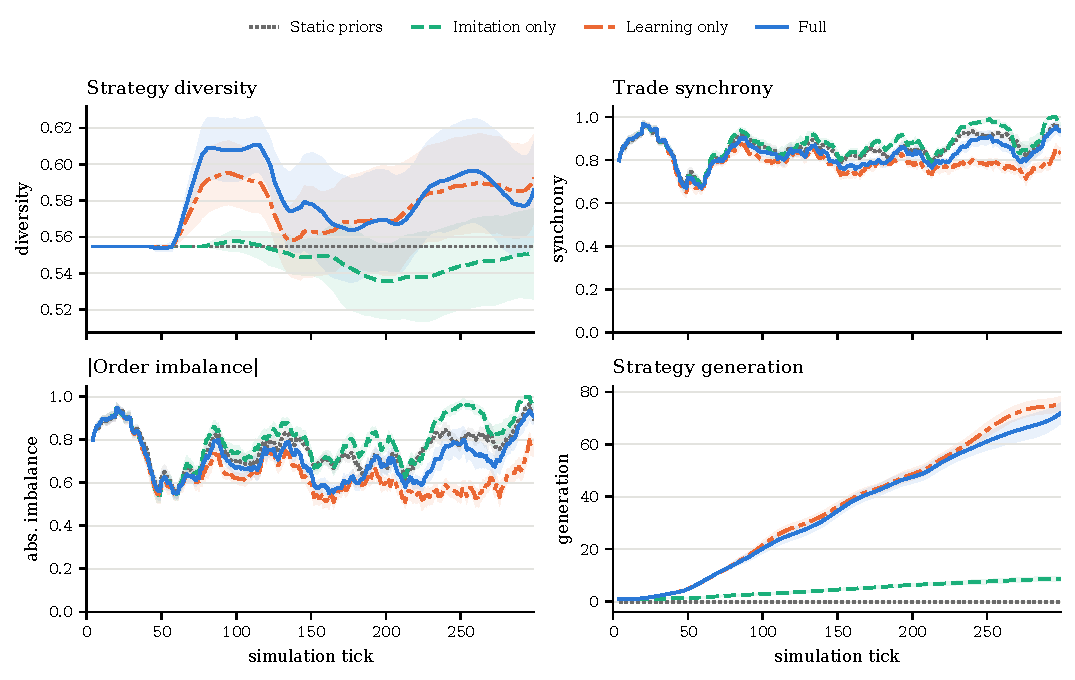
\includegraphics[width=\linewidth]{figures/fig_dynamics.pdf}
  \caption{Discovery-window trajectories (20-tick rolling means, 95\% confidence
  intervals across 16 seeds). Learning raises strategy diversity and generation
  and reduces trade synchrony; imitation alone raises synchrony and leaves
  diversity near the static baseline. The full system sits between the two.}
  \label{fig:dynamics}
\end{figure}

\subsection{Multi-window replication: what survives}

The held-out windows tell a more selective story. Figure~\ref{fig:windows} and
Table~\ref{tab:replication} compare discovery and held-out effects. Three results
survive. First, learning increases strategy diversity by $0.107$ (95\% CI
$[0.093,0.121]$) and the full system by $0.122$ ($[0.091,0.147]$); $94$--$96\%$
of the 48 paired observations are positive (both $p<10^{-8}$). Second, imitation
increases trade synchrony by $0.020$ ($[0.013,0.028]$) and $|$imbalance$|$ by
$0.041$ ($[0.030,0.053]$); $90\%$ and $98\%$ of paired observations are positive
(both $p<10^{-10}$). Third, the full system is more coordinated than learning
alone: synchrony $+0.022$ and imbalance $+0.047$ (both $p<10^{-8}$), with a
small return advantage ($+0.037$ pp, $p=.038$) but no drawdown advantage.

What does not survive is the performance story. Full minus static return is
$-0.019$ pp (95\% CI $[-0.081,+0.043]$, $p=.56$); the drawdown improvement is
$-0.034$ pp (i.e.\ drawdowns are $0.034$ pp larger; $p=.15$). Learning-only is
$0.056$ pp \emph{worse} than static ($p=.005$) and its drawdown improvement is
$-0.028$ pp (raw $p=.047$, not Holm-corrected). Imitation-only is statistically
indistinguishable from static on return ($-0.018$ pp, $p=.79$), raises
coordination, and increases drawdown magnitude by $0.061$ pp ($p=.005$). The
discovery-window signs for full-minus-static return and synchrony reverse:
$+0.110$ pp and $-0.022$ in discovery become $-0.019$ pp and $+0.016$ in
held-out. The full system's return advantage over learning alone is real but
small; it does not translate into a drawdown advantage, and it does not make the
full system better than static priors on average.

\begin{figure}[t]
  \centering
  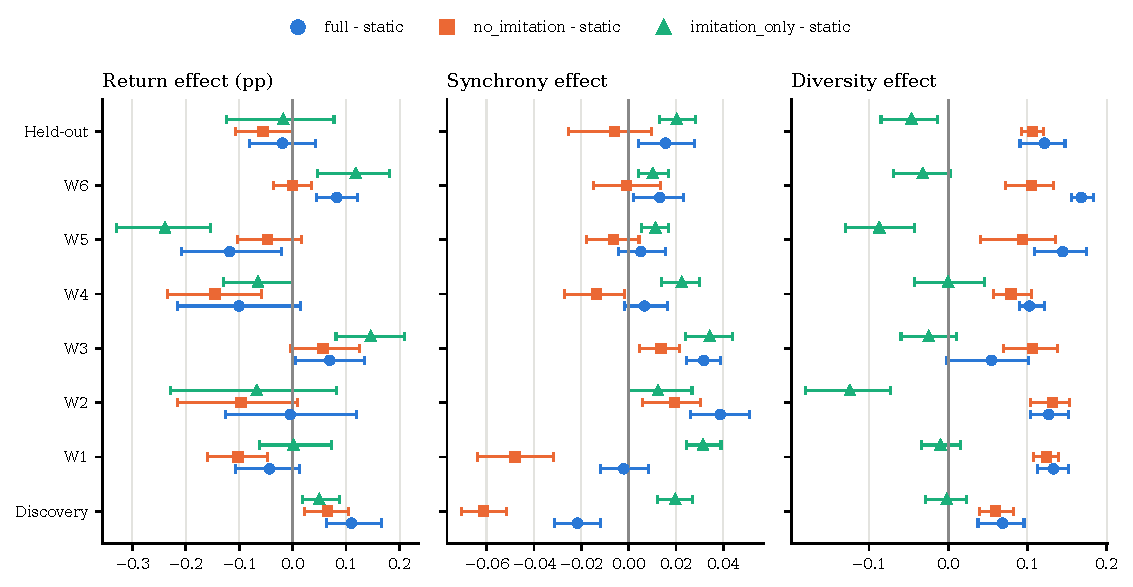
\includegraphics[width=\linewidth]{figures/fig_windows_forest.pdf}
  \caption{Per-window and pooled effects relative to static priors. Each row is
  one window; the top row pools the six held-out windows with a window-cluster
  bootstrap. Return and synchrony/diversity are shown. The discovery window
  (bottom row) has a positive full/learning return effect and a negative
  full/learning synchrony effect; the held-out pooled effects reverse the return
  sign and the full-system synchrony sign, while the diversity gain and the
  imitation coordination effect persist.}
  \label{fig:windows}
\end{figure}

\begin{table}[t]
  \centering
  \small
  \setlength{\tabcolsep}{3pt}
  \caption{Discovery versus held-out paired effects. Entries are mean differences
  (condition minus static) in percentage points for return and drawdown
  improvement (positive drawdown improvement means a smaller drawdown) and
  unitless for diversity, synchrony, and $|$imbalance$|$. Discovery uses 16
  seeds and Holm-adjusted $p$; held-out pools 48 seed-window pairs across six
  windows with a window-cluster bootstrap. Stars: $^{*}p<.05$, $^{**}p<.01$,
  $^{***}p<.001$ (held-out raw; discovery Holm). The held-out drawdown difference
  for learning-only is raw $p=.047$ and does not survive Holm correction.}
  \label{tab:replication}
  \begin{tabular}{lcccccc}
    \toprule
    & \multicolumn{2}{c}{Full $-$ Static} & \multicolumn{2}{c}{Learning $-$ Static} & \multicolumn{2}{c}{Imitation $-$ Static}\\
    \cmidrule(lr){2-3}\cmidrule(lr){4-5}\cmidrule(lr){6-7}
    Metric & Discovery & Held-out & Discovery & Held-out & Discovery & Held-out\\
    \midrule
    Return (pp) & $+0.110^{***}$ & $-0.019$ & $+0.065^{*}$ & $-0.056^{**}$ & $+0.050^{*}$ & $-0.018$\\
    Drawdown improvement (pp) & $+0.084^{**}$ & $-0.034$ & $+0.163^{***}$ & $-0.028^{*}$ & $-0.009$ & $-0.061^{**}$\\
    Strategy diversity & $+0.069^{**}$ & $+0.122^{***}$ & $+0.060^{**}$ & $+0.107^{***}$ & $-0.002$ & $-0.046^{***}$\\
    Trade synchrony & $-0.022^{**}$ & $+0.016^{***}$ & $-0.061^{***}$ & $-0.006$ & $+0.020^{***}$ & $+0.020^{***}$\\
    $|$Order imbalance$|$ & $-0.043^{**}$ & $+0.033^{***}$ & $-0.114^{***}$ & $-0.014$ & $+0.041^{***}$ & $+0.041^{***}$\\
    \bottomrule
  \end{tabular}
\end{table}

\subsection{Strategy divergence and guild lineage}

Figure~\ref{fig:strategy} makes the divergence mechanism visible. At tick 0 all
conditions have the same mean pairwise signal-genome distance ($0.157$). Static
priors stay exactly flat. Learning-only rises to $0.320$ by tick 300; the full
system rises to $0.254$, because imitation pulls it back toward the population;
imitation-only falls to $0.118$, i.e.\ it homogenizes. The guild-diversity index
tells a related but not identical story: full $0.624$, learning-only $0.615$,
imitation-only $0.553$, static $0.555$. The full system keeps high guild
diversity while reducing continuous genome distance: imitation helps agents cross
guild boundaries but also blends their playbooks. At the end of the discovery
window, $19.9\%$ of full agents, $16.0\%$ of learning-only agents, $10.6\%$ of
imitation-only agents, and $0\%$ of static agents have a different final guild;
the fractions that ever switch are $30.9\%$, $21.1\%$, $12.9\%$, and $0\%$
(10-tick samples). The full system therefore has the most lineage churn, even
though it is not the most genomically diverse.

\begin{figure}[t]
  \centering
  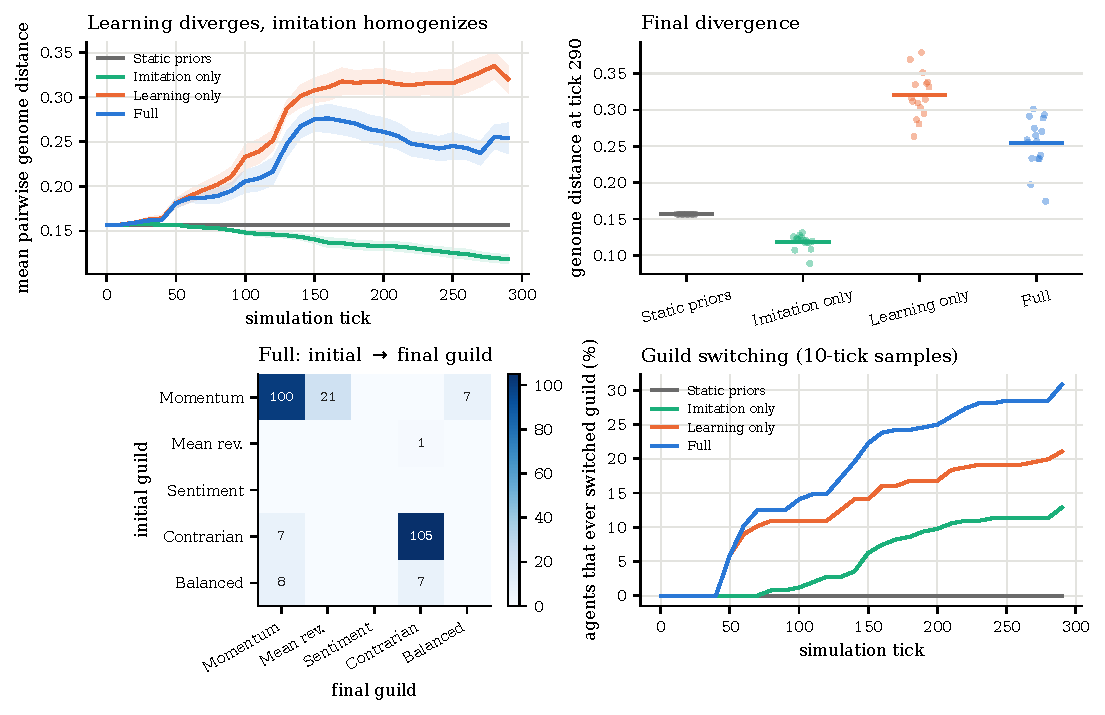
\includegraphics[width=\linewidth]{figures/fig_strategy_dynamics.pdf}
  \caption{Signal-genome divergence and guild lineage in the discovery window.
  Top left: mean pairwise distance over the six normalized signal weights;
  learning diverges, imitation homogenizes, and the full system balances. Top
  right: final distance by condition. Bottom left: full-system initial-to-final
  guild transition matrix. Bottom right: fraction of agents that ever switched
  guild in the 10-tick strategy snapshots. Guild switching is not the same as
  final divergence: the full system mixes guilds while imitation compresses the
  continuous genome.}
  \label{fig:strategy}
\end{figure}

\subsection{The learning--imitation phase map}

Figure~\ref{fig:phase} reports the 4$\times$4 sweep on the discovery window.
Coordination rises monotonically with imitation at every learning scale, and
learning lowers synchrony at every imitation scale. Return and drawdown are
non-monotone. At $1\times$ learning, return is best at $0.5\times$ imitation
($-1.061\%$) and deteriorates at $1\times$ ($-1.121\%$) and $2\times$
($-1.167\%$); drawdown magnitude follows the same ordering ($1.305\%$,
$1.355\%$, $1.388\%$). The best cell in the sweep is learning $1\times$,
imitation $0.5\times$; the worse corners are no learning and high imitation.
Strategy diversity increases with learning ($0.547$ at $0\times$ to
$0.653$--$0.662$ at $2\times$), and at $1\times$ learning it also increases with
imitation ($0.578$ to $0.635$), reflecting guild mixing. Exposure falls modestly
with learning ($33.0\%$ at zero learning to $32.3\%$ at $0.5\times$ and
$31.7\%$ at $1\times$) and rises slightly with imitation. The phase map is a discovery-window result; its qualitative
lesson is that coordination is not performance. A designer who maximizes
synchrony would choose high imitation; a designer who maximizes return or
drawdown in this window chooses moderate imitation.

\begin{figure}[t]
  \centering
  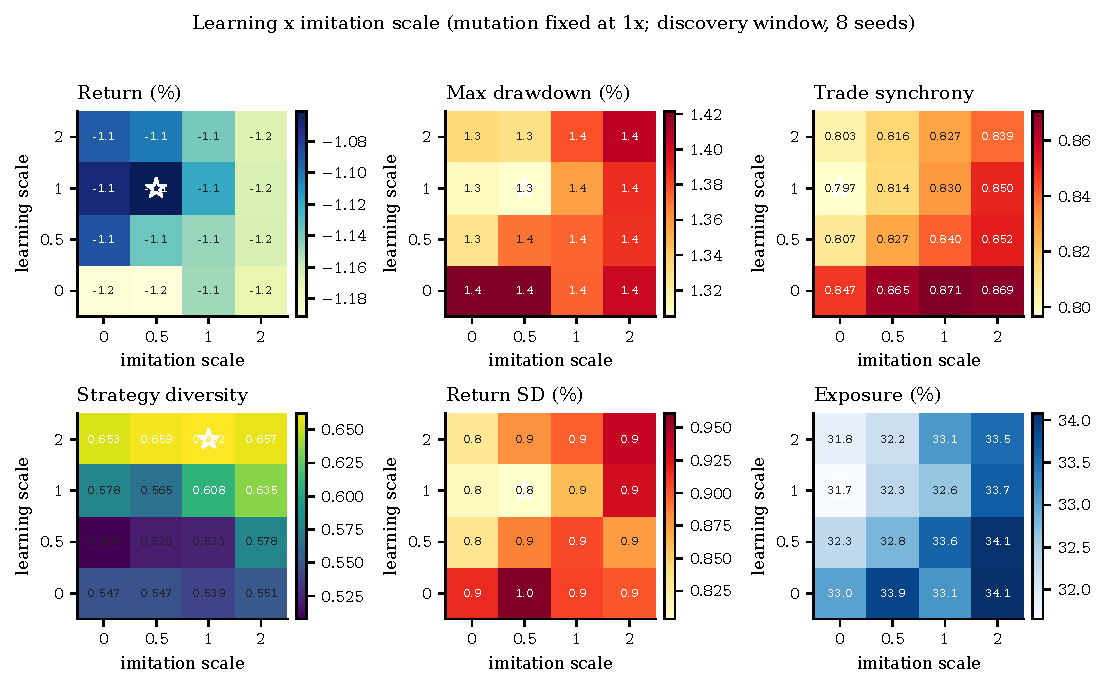
\includegraphics[width=\linewidth]{figures/fig_phase_map.pdf}
  \caption{Learning $\times$ imitation phase map on the discovery window (8
  seeds, 250 ticks, mutation fixed at $1\times$). Return, drawdown, synchrony,
  diversity, return dispersion, and exposure are shown. The star marks the best
  cell for the metric (higher return/diversity, lower drawdown/synchrony/return
  SD/exposure). Coordination rises monotonically with imitation; return and
  drawdown peak at moderate imitation and worsen at high imitation.}
  \label{fig:phase}
\end{figure}

\subsection{Exposure, benchmarks, and the missing alpha}

Figure~\ref{fig:benchmark} explains why the discovery-window return result
should not be read as alpha. The agents hold only about $32\%$ of their equity in
stocks on average; the rest is cash. The equal-weight market return ranges from
$-1.40\%$ in the discovery window to $+1.97\%$ in W6. Agent returns are compressed
toward zero: in the discovery window the full system returns $-0.19\%$ while the
market returns $-1.40\%$, but its mean exposure-implied return is about
$-0.48\%$; the difference is timing/selection and fees, not a fully invested
outperformance. In W5 the market rises $+1.06\%$ while the full system loses
$-0.76\%$ (its exposure is $33.7\%$), a large adverse residual. In W6 the market
rises $+1.97\%$ and the full system earns $+0.45\%$ (exposure $25.8\%$). The
conditions differ by a few tenths of a percentage point, while the market moves
by several percentage points. The correct conclusion is that the agents are
cash-heavy and regime-sensitive; their low exposure explains most of the gap to
the market, while the small condition differences are not a robust alpha.

\begin{figure}[t]
  \centering
  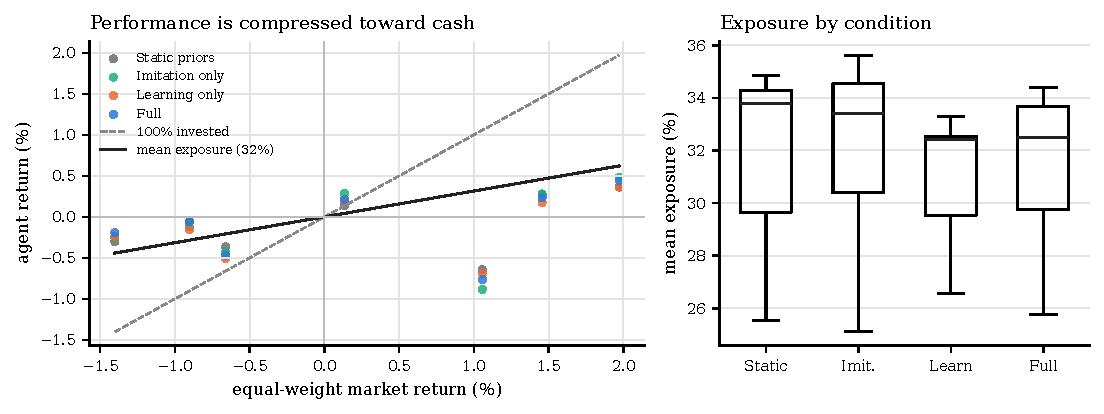
\includegraphics[width=\linewidth]{figures/fig_benchmark.pdf}
  \caption{Performance is compressed toward cash. Left: equal-weight market
  return versus agent return for every window and condition; the dashed line is
  $100\%$ invested and the solid line is the mean exposure ($32\%$). Right: mean
  exposure by condition. The agents take only about one third of the market move;
  condition differences are small relative to the market and are not an alpha
  claim.}
  \label{fig:benchmark}
\end{figure}

\subsection{Observer audit: coordination is not a crash warning}

The observer audit is the most cautionary part of the paper. On the discovery
window, the original composite score is uninformative: run-level correlations
with future synchrony, $|$imbalance$|$, and $|$drawdown$|$ are $0.029$, $0.044$,
and $-0.133$ ($p=.30$ for drawdown). Its polarization term is negatively
associated with future $|$drawdown$|$ ($\rho=-0.546$), the opposite of its risk
label: a split town is less likely to suffer a correlated drawdown. The v2
flow-risk score is strongly associated with future synchrony ($\rho=.754$),
$|$imbalance$|$ ($.769$), and $|$drawdown$|$ ($.609$) on the same window; the
run-level AUC for high future $|$drawdown$|$ is $.805$. This is the result that
motivated a risk narrative.

The held-out windows separate prediction from persistence. The v2 flow score
still predicts future synchrony ($\rho=.592$) and $|$imbalance$|$ ($.603$;
$p<10^{-18}$), so it is a genuine coordination-persistence signal. But its
correlation with future $|$drawdown$|$ is $-0.041$ ($p=.58$), and the run-level
AUC for high future $|$drawdown$|$ is $.443$---below chance. The event-level AUC
is $.532$ (95\% CI $[.512,.554]$), effectively no discrimination. The original
composite's held-out drawdown correlation is $+0.305$ and polarization's is
$+0.580$; both have the opposite sign from the discovery window. In other words,
the component that looked protective in one window looks risky in another, and
the flow score that looked like an early warning in one window does not warn on
the others. Table~\ref{tab:observer} and Figure~\ref{fig:observer} report the
details.

\begin{table}[t]
  \centering
  \small
  \setlength{\tabcolsep}{3pt}
  \caption{Observer audit. Panel A: run-level Spearman correlations with future
  outcomes. Panel B: AUC for high future $|$drawdown$|$ (top quartile), at the
  run level (one maximum future drawdown per run) and the event level (one
  observation per report). Discovery $n=64$ runs; held-out $n=192$ runs. The v2
  score is fixed before the held-out evaluation; no re-fitting. The same score
  predicts coordination in both samples but its drawdown signal reverses.}
  \label{tab:observer}
  \begin{tabular}{lccc}
    \toprule
    \multicolumn{4}{l}{\emph{Panel A: run-level correlations}}\\
    Predictor & Future synchrony & Future $|$imbalance$|$ & Future $|$drawdown$|$\\
    \midrule
    v2 flow (discovery) & $0.754$ & $0.769$ & $0.609$\\
    v2 flow (held-out) & $0.592$ & $0.603$ & $-0.041$ ($p=.58$)\\
    v1 composite (discovery) & $0.029$ & $0.044$ & $-0.133$\\
    v1 composite (held-out) & $-0.039$ & $-0.059$ & $+0.305$\\
    Polarization (discovery) & $-0.556$ & $-0.540$ & $-0.546$\\
    Polarization (held-out) & $-0.206$ & $-0.213$ & $+0.580$\\
    \bottomrule
  \end{tabular}\\[4pt]
  \begin{tabular}{lcccc}
    \toprule
    \multicolumn{5}{l}{\emph{Panel B: AUC for high future $|$drawdown$|$}}\\
    Predictor & Run-level, discovery & Run-level, held-out & Event, discovery & Event, held-out\\
    \midrule
    v2 flow & $0.805$ & $0.443$ & $0.566$ & $0.532$\\
    v1 composite & $0.522$ & $0.523$ & $0.516$ & $0.489$\\
    Polarization & $0.283$ & $0.733$ & $0.475$ & $0.484$\\
    \bottomrule
  \end{tabular}
\end{table}

\begin{figure}[t]
  \centering
  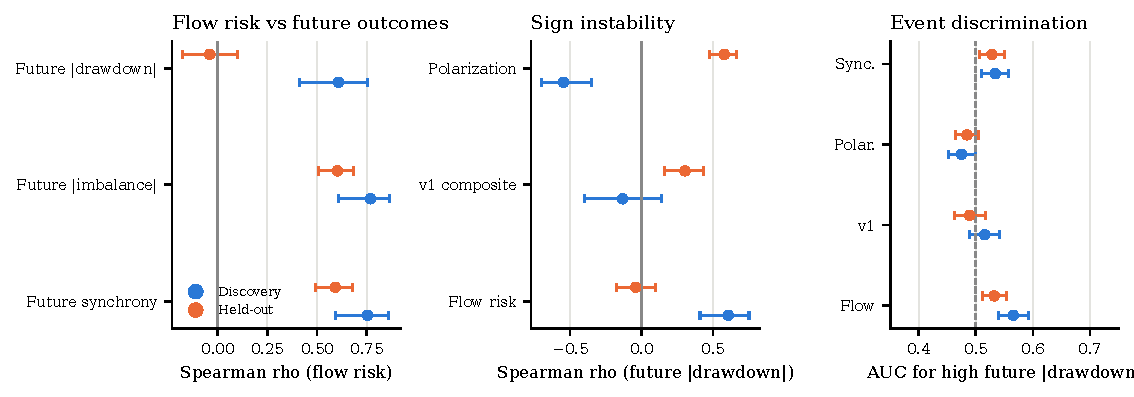
\includegraphics[width=\linewidth]{figures/fig_observer_oos.pdf}
  \caption{Observer out-of-sample audit. Left: v2 flow risk versus future
  synchrony, $|$imbalance$|$, and $|$drawdown$|$ on the discovery and held-out
  windows. Middle: correlations with future $|$drawdown$|$ for the v1 composite,
  polarization, and flow risk; the signs are unstable across windows. Right:
  AUC for high future $|$drawdown$|$ at the run level; the v2 flow score falls
  from $.81$ in discovery to $.44$ in held-out. Flow alignment predicts
  coordination, not drawdown.}
  \label{fig:observer}
\end{figure}

The practical lesson is not that observers are useless. The Physicist and
Mathematician fields are descriptive and useful; the flow score is a useful
measure of order-flow alignment. The lesson is that a scalar labelled ``risk''
must be validated against the outcome it claims to predict, on held-out windows,
at both run and event levels. A run-level correlation can be driven by
between-run heterogeneity; an event-level AUC asks whether a report is an early
warning. The v2 score is a coordination-persistence signal, not a validated crash
warning. The interactive application now labels the field ``flow-alignment
risk'' rather than ``cascade risk'' to reflect this distinction.

\subsection{The imitation network}

Figure~\ref{fig:network} and Table~\ref{tab:network} describe the social
transmission layer. The full condition records 596 imitation events over 16 runs
(37.3 per run); imitation-only records 585 (36.6 per run). All 16 agents appear
as both teachers and learners. Effective teacher concentration is low
($14.0$ of 16), mean trust on an imitation edge is $0.118$, and teachers are
slightly fitter than learners (mean fitness gap $+0.0045$). Only $7.2\%$ of full
imitation events change the learner's guild; imitation usually adjusts weights
within a guild. The most common locations are the Guild Hall ($114$ events),
Morning Brew Cafe ($93$), Town Square ($70$), market ($57$), Rumor Mill ($56$),
and Quant Lab ($34$). The new social hubs matter: imitation is concentrated in
places where agents meet, not in a single guru's broadcast. The network is
diffuse, trust- and fitness-gated, and embedded in the town's geography.

\begin{figure}[t]
  \centering
  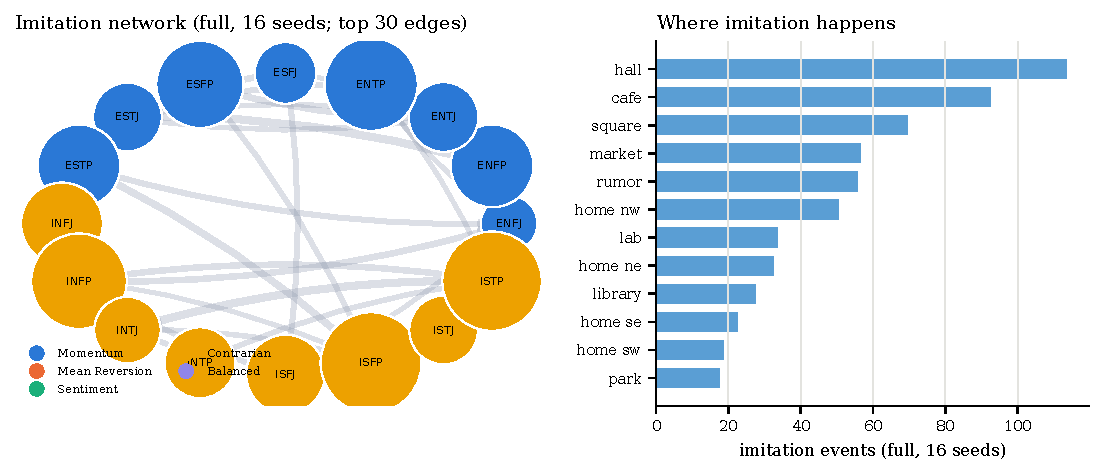
\includegraphics[width=\linewidth]{figures/fig_network.pdf}
  \caption{Imitation network and geography (full condition, 16 seeds). Left:
  aggregate teacher-to-learner edges (top 30) with node colour by modal final
  guild and node size by teacher in-degree. Right: imitation events by location.
  Transmission is diffuse rather than guru-driven; the Guild Hall, cafe, square,
  market, and Rumor Mill are the main sites.}
  \label{fig:network}
\end{figure}

\begin{table}[t]
  \centering
  \small
  \caption{Imitation-network summary (discovery window, 16 seeds). ``Effective
  teachers'' is $1/\sum_i s_i^2$ for teacher in-degree shares $s_i$. The fitness
  gap is teacher minus learner fitness at the event.}
  \label{tab:network}
  \begin{tabular}{lcccccc}
    \toprule
    Condition & Events & Events/run & Effective teachers & Mean trust & Fitness gap & Guild change\\
    \midrule
    Full & 596 & 37.3 & 14.0 & 0.118 & $+0.0045$ & $7.2\%$\\
    Imitation only & 585 & 36.6 & 13.9 & 0.115 & $+0.0044$ & $10.4\%$\\
    Learning only & 0 & 0 & -- & -- & -- & --\\
    Static priors & 0 & 0 & -- & -- & -- & --\\
    \bottomrule
  \end{tabular}
\end{table}

\section{Discussion}

The central empirical pattern is a separation between behavioural mechanisms and
economic outcomes. Learning is a diversifying force. It gives agents different
experiences, moves their signal genomes apart, and raises guild diversity; in the
discovery window it also lowers synchrony and improves downside outcomes. The
diversification result replicates across all six held-out windows. Imitation is a
coordinating force. It raises trade synchrony and order-flow imbalance, and the
effect replicates across all six held-out windows with high sign consistency. The
full system is a balance: it is more diverse than static priors and more
coordinated than learning alone. The phase map shows that coordination can be
increased monotonically by raising imitation, while return and drawdown are best
at moderate imitation and deteriorate at high imitation.

The performance result is fragile. The discovery window is a down/high-volatility
week; learning and the full system lose less than static priors because they are
cash-heavy, not because they have a robust alpha. Across six held-out windows the
full-minus-static return difference is statistically indistinguishable from zero
and the drawdown difference is slightly negative. Learning-only actually
underperforms static priors on average. The agents hold about one third of their
equity in stocks, so their returns are a compressed image of the market; the
condition differences are small relative to the market moves. This is a useful
caution for agent-based market papers: a single window can make a risk-reduction
story look like a performance result.

The observer result is the sharpest caution. The v1 composite had a coherent
narrative and failed. The v2 flow score had a strong discovery-window drawdown
correlation and a run-level AUC of $.81$, but the correlation reversed on held-out
windows and the run-level AUC fell to $.44$. The flow score's coordination
prediction survived ($\rho\approx.59$--$.60$), which is exactly what a
coordination-persistence measure should do; it is not a crash warning. The
polarization term changed sign across windows. These are not small-sample
quibbles: they are the difference between a metric that describes the current
state and a metric that forecasts the outcome one cares about. Observer research
should report the outcome-specific, held-out, run-level and event-level results,
not only the in-sample correlation.

The imitation network adds a social-layer result. Transmission is diffuse: all
sixteen agents teach and learn, effective teacher concentration is low, and the
fitness gap is small. The town's geography matters: the Guild Hall, cafe, square,
market, and Rumor Mill are the main sites. Imitation usually adjusts weights
within a guild; guild changes are rare. The full system has more lineage churn
than learning alone, because imitation helps agents cross guild boundaries, but
it also compresses continuous genome distance. This is a plausible mechanism for
the full system's combination of high guild diversity and lower genome distance
than learning-only.

\section{Limitations}

\begin{itemize}
  \item \textbf{Seven windows, two months, five mega-caps.} The six held-out
  windows are not a random sample; they were chosen from the available 60-day
  five-minute history to span regimes. The discovery window is a down/high-vol
  week. Other assets, frequencies, and longer samples may differ.
  \item \textbf{Exogenous prices.} The House absorbs residual order flow, so the
  town price equals the replay price. This isolates behaviour but removes
  endogenous price impact, feedback, and liquidity effects.
  \item \textbf{Long-only, cash-heavy agents.} Five symbols, no shorting,
  leverage, options, borrow costs, or volume limits. Mean exposure is about
  $32\%$; the performance comparisons are not a test of a fully invested
  strategy.
  \item \textbf{Rule-based agents and observers.} The learning rule is a
  lightweight reward-modulated Hebbian update, not deep reinforcement learning;
  imitation is a fixed blend; observers are heuristics. LLM enrichment was
  disabled. The results may differ with richer agents.
  \item \textbf{Post-hoc v2 and selected windows.} The v2 formula was motivated by
  the discovery-window v1 failure. The held-out windows were not used to fit it,
  but they were fetched after the formula was fixed and selected by regime. The
  out-of-sample test is temporal and formula-fixed, not a pre-registered random
  sample.
  \item \textbf{Multiple comparisons.} The held-out tests are reported raw; the
  strong behavioural effects survive Holm correction, but the small performance
  differences should not be over-interpreted.
  \item \textbf{Outcome definitions.} The run-level AUC uses one maximum future
  drawdown per run; the event-level AUC uses overlapping 20-tick windows. Both
  answer useful questions but neither is a full early-warning evaluation with
  lead-time constraints.
  \item \textbf{No financial claim.} This is a simulation, not investment advice,
  and the returns are not an alpha claim.
\end{itemize}

\section{Conclusion}

A multi-window, multi-seed agent-based market study can separate robust
behavioural mechanisms from fragile performance and observer claims. Learning
diverges: it moves strategy genomes apart and raises guild diversity, and this
survives six held-out windows. Imitation coordinates: it raises trade synchrony
and order-flow imbalance, and this also survives. The full system balances the
two, but it does not deliver a robust return or drawdown advantage; the agents
are cash-heavy and the discovery-window risk reduction is mostly exposure. The
learning--imitation phase map shows that coordination rises monotonically with
imitation while performance peaks at moderate imitation. The observer audit shows
that a flow-based score can predict coordination in and out of sample while
failing as a drawdown warning; its discovery-window drawdown signal reverses out
of sample, and polarization's sign is unstable. Agent-based market simulations
are most useful as behavioural laboratories when they report coordination and
diversity explicitly, freeze and validate their data, hold out whole market
windows, and evaluate observer scalars against the outcome they claim to predict
at both run and event levels.

\section*{Data and code availability}

Code, the seven frozen snapshots, the experiment runner, the analysis scripts,
and all figures are available at
\url{https://github.com/huiihao/agent-street}. The discovery snapshot SHA-256 is
\texttt{3c9cf0ff864b68e6886c1f3181f67e6}\allowbreak
\texttt{e93dbacef8102007c34fedc768c9f86fe}; each held-out snapshot has a
metadata file with its SHA-256. Reproduction:
\begin{verbatim}
python experiments/run_experiment.py --design base --ticks 300 \
  --seeds 1,...,16 --out experiments/results
python experiments/run_experiment.py --design base --ticks 300 \
  --seeds 1,...,8 --snapshot <window>/market_snapshot_5m_5d.json \
  --metadata <window>/snapshot_metadata.json --out experiments/results_windows/<window>
python experiments/run_experiment.py --design sweep --ticks 250 \
  --seeds 1,...,8 --learning-scales 0,0.5,1,2 \
  --imitation-scales 0,0.5,1,2 --out experiments/results_sweep
python experiments/analyze_results.py
python experiments/analyze_extensions.py
python experiments/analyze_strategy.py
python -m unittest discover -s tests -v
\end{verbatim}

\bibliographystyle{plainnat}
\bibliography{refs}

\end{document}
